\documentclass{article}

% ICLR 2027 submission.  \iclrfinalcopy MUST stay commented out: the style file
% hardcodes "Anonymous authors / Paper under double-blind review" in the
% non-final branch, so author identity never reaches the compiled PDF.
\usepackage{iclr2027_conference,times}

\usepackage[utf8]{inputenc}
\usepackage[T1]{fontenc}
\usepackage{hyperref}
\usepackage{url}
\usepackage{booktabs}
\usepackage{adjustbox}
\usepackage{amsfonts}
\usepackage{nicefrac}
\usepackage{microtype}
\usepackage{xcolor}
\usepackage{graphicx}
\usepackage{tikz}
\usepackage{pgfplots}
\pgfplotsset{compat=1.18}
\usetikzlibrary{arrows.meta,positioning,calc,patterns}

\usepackage{multirow}
\usepackage{siunitx}
\sisetup{detect-weight=true,detect-inline-weight=math}

\input{math_commands.tex}

% Appendix-aware cross-reference: \secref would print "section A" for an appendix
% label, which reads wrong.
\newcommand{\appref}[1]{Appendix~\ref{#1}}

% Every number in the prose is a macro defined here.  This must be read in the
% PREAMBLE: \newcommand has to be defined before the section files that use it
% are tokenised, otherwise the references resolve to undefined control sequences.
% GENERATED by scripts/paper/make_tables.py -- do not edit by hand.
\newcommand{\BaseNativeN}{20}
\newcommand{\BaseFallbackN}{28}
\newcommand{\BaseNativeRate}{85.0\%}
\newcommand{\BaseFallbackRate}{28.6\%}
\newcommand{\BasePooledRate}{52.1\%}
\newcommand{\BaselineSwing}{32.9}
\newcommand{\ResWebDomMissingCtlMargNat}{84.4\%}
\newcommand{\ResWebDomMissingFltMargNat}{78.8\%}
\newcommand{\ResWebDomMissingCtlMargNatN}{32}
\newcommand{\ResWebDomMissingFltMargNatN}{33}
\newcommand{\ResWebPopupBlockCtlMargNat}{69.7\%}
\newcommand{\ResWebPopupBlockFltMargNat}{77.4\%}
\newcommand{\ResWebPopupBlockCtlMargNatN}{33}
\newcommand{\ResWebPopupBlockFltMargNatN}{31}
\newcommand{\ResWebHttpErrorCtlMargNat}{71.9\%}
\newcommand{\ResWebHttpErrorFltMargNat}{73.5\%}
\newcommand{\ResWebHttpErrorCtlMargNatN}{32}
\newcommand{\ResWebHttpErrorFltMargNatN}{34}
\newcommand{\ResWebTimeoutCtlMargNat}{78.8\%}
\newcommand{\ResWebTimeoutFltMargNat}{81.2\%}
\newcommand{\ResWebTimeoutCtlMargNatN}{33}
\newcommand{\ResWebTimeoutFltMargNatN}{32}
\newcommand{\ResAgentParamErrorCtlMargNat}{93.9\%}
\newcommand{\ResAgentParamErrorFltMargNat}{80.6\%}
\newcommand{\ResAgentParamErrorCtlMargNatN}{33}
\newcommand{\ResAgentParamErrorFltMargNatN}{31}
\newcommand{\ResWebDomMissingDelta}{$-$2.5}
\newcommand{\ResWebDomMissingP}{1.000}
\newcommand{\ResWebDomMissingCtl}{67.5\%}
\newcommand{\ResWebDomMissingFlt}{65.0\%}
\newcommand{\ResWebDomMissingN}{40}
\newcommand{\ResWebDomMissingDisc}{15}
\newcommand{\ResWebPopupBlockDelta}{$+$2.5}
\newcommand{\ResWebPopupBlockP}{1.000}
\newcommand{\ResWebPopupBlockCtl}{57.5\%}
\newcommand{\ResWebPopupBlockFlt}{60.0\%}
\newcommand{\ResWebPopupBlockN}{40}
\newcommand{\ResWebPopupBlockDisc}{11}
\newcommand{\ResWebHttpErrorDelta}{$+$5.0}
\newcommand{\ResWebHttpErrorP}{0.774}
\newcommand{\ResWebHttpErrorCtl}{57.5\%}
\newcommand{\ResWebHttpErrorFlt}{62.5\%}
\newcommand{\ResWebHttpErrorN}{40}
\newcommand{\ResWebHttpErrorDisc}{12}
\newcommand{\ResWebTimeoutDelta}{$+$0.0}
\newcommand{\ResWebTimeoutP}{1.000}
\newcommand{\ResWebTimeoutCtl}{65.0\%}
\newcommand{\ResWebTimeoutFlt}{65.0\%}
\newcommand{\ResWebTimeoutN}{40}
\newcommand{\ResWebTimeoutDisc}{6}
\newcommand{\ResAgentParamErrorDelta}{$-$15.0}
\newcommand{\ResAgentParamErrorP}{0.070}
\newcommand{\ResAgentParamErrorCtl}{77.5\%}
\newcommand{\ResAgentParamErrorFlt}{62.5\%}
\newcommand{\ResAgentParamErrorN}{40}
\newcommand{\ResAgentParamErrorDisc}{8}
\newcommand{\ResWebDomMissingDeltaNat}{$-$6.7}
\newcommand{\ResWebDomMissingPNat}{0.754}
\newcommand{\ResWebDomMissingCtlNat}{83.3\%}
\newcommand{\ResWebDomMissingFltNat}{76.7\%}
\newcommand{\ResWebDomMissingNNat}{30}
\newcommand{\ResWebDomMissingDiscNat}{10}
\newcommand{\ResWebPopupBlockDeltaNat}{$+$9.7}
\newcommand{\ResWebPopupBlockPNat}{0.508}
\newcommand{\ResWebPopupBlockCtlNat}{67.7\%}
\newcommand{\ResWebPopupBlockFltNat}{77.4\%}
\newcommand{\ResWebPopupBlockNNat}{31}
\newcommand{\ResWebPopupBlockDiscNat}{9}
\newcommand{\ResWebHttpErrorDeltaNat}{$+$0.0}
\newcommand{\ResWebHttpErrorPNat}{1.000}
\newcommand{\ResWebHttpErrorCtlNat}{71.0\%}
\newcommand{\ResWebHttpErrorFltNat}{71.0\%}
\newcommand{\ResWebHttpErrorNNat}{31}
\newcommand{\ResWebHttpErrorDiscNat}{8}
\newcommand{\ResWebTimeoutDeltaNat}{$+$3.2}
\newcommand{\ResWebTimeoutPNat}{1.000}
\newcommand{\ResWebTimeoutCtlNat}{77.4\%}
\newcommand{\ResWebTimeoutFltNat}{80.6\%}
\newcommand{\ResWebTimeoutNNat}{31}
\newcommand{\ResWebTimeoutDiscNat}{3}
\newcommand{\ResAgentParamErrorDeltaNat}{$-$12.9}
\newcommand{\ResAgentParamErrorPNat}{0.219}
\newcommand{\ResAgentParamErrorCtlNat}{93.5\%}
\newcommand{\ResAgentParamErrorFltNat}{80.6\%}
\newcommand{\ResAgentParamErrorNNat}{31}
\newcommand{\ResAgentParamErrorDiscNat}{6}
\newcommand{\OfficialN}{400}
\newcommand{\OfficialNativeN}{324}
\newcommand{\OfficialFallbackN}{76}
\newcommand{\OfficialNativePairs}{154}
\newcommand{\OfficialAllPairs}{200}
\newcommand{\MdePairedNForty}{19.2}
\newcommand{\MdePairedNEighty}{13.8}
\newcommand{\MdePairedNOneFiveFive}{10}
\newcommand{\PairsForTenPP}{155}
\newcommand{\PiDAll}{0.260}
\newcommand{\PiDNative}{0.234}
\newcommand{\PairsForTenPPObserved}{181}
\newcommand{\PairsForTenPPObservedAll}{202}
\newcommand{\BehWebDomMissingStepDelta}{$-$0.10}
\newcommand{\BehWebDomMissingStepHL}{$+$0.0}
\newcommand{\BehWebDomMissingStepP}{0.956}
\newcommand{\BehWebDomMissingTimeDelta}{$-$66.1}
\newcommand{\BehWebDomMissingTimeHL}{$-$46.0}
\newcommand{\BehWebDomMissingTimeP}{0.068}
\newcommand{\BehWebDomMissingN}{80}
\newcommand{\BehWebPopupBlockStepDelta}{$-$0.44}
\newcommand{\BehWebPopupBlockStepHL}{$+$0.0}
\newcommand{\BehWebPopupBlockStepP}{0.509}
\newcommand{\BehWebPopupBlockTimeDelta}{$-$27.5}
\newcommand{\BehWebPopupBlockTimeHL}{$-$21.8}
\newcommand{\BehWebPopupBlockTimeP}{0.004}
\newcommand{\BehWebPopupBlockN}{80}
\newcommand{\BehWebHttpErrorStepDelta}{$+$4.22}
\newcommand{\BehWebHttpErrorStepHL}{$+$4.0}
\newcommand{\BehWebHttpErrorStepP}{$<$0.001}
\newcommand{\BehWebHttpErrorTimeDelta}{$+$149.9}
\newcommand{\BehWebHttpErrorTimeHL}{$+$132.3}
\newcommand{\BehWebHttpErrorTimeP}{$<$0.001}
\newcommand{\BehWebHttpErrorN}{80}
\newcommand{\BehWebTimeoutStepDelta}{$-$0.72}
\newcommand{\BehWebTimeoutStepHL}{$-$0.5}
\newcommand{\BehWebTimeoutStepP}{0.021}
\newcommand{\BehWebTimeoutTimeDelta}{$-$13.2}
\newcommand{\BehWebTimeoutTimeHL}{$-$8.9}
\newcommand{\BehWebTimeoutTimeP}{0.316}
\newcommand{\BehWebTimeoutN}{80}
\newcommand{\BehAgentParamErrorStepDelta}{$+$2.30}
\newcommand{\BehAgentParamErrorStepHL}{$+$1.5}
\newcommand{\BehAgentParamErrorStepP}{$<$0.001}
\newcommand{\BehAgentParamErrorTimeDelta}{$+$20.6}
\newcommand{\BehAgentParamErrorTimeHL}{$+$7.1}
\newcommand{\BehAgentParamErrorTimeP}{0.460}
\newcommand{\BehAgentParamErrorN}{80}
\newcommand{\NoiseFloorLo}{103.7}
\newcommand{\NoiseFloorHi}{224.6}
\newcommand{\NoiseFloorRatio}{2.17}
\newcommand{\ResHttpErrorStepDelta}{$+$4.22}
\newcommand{\ResHttpErrorTimeDelta}{$+$149.9}
\newcommand{\ResParamErrStepDelta}{$+$2.30}
\newcommand{\ArchReactCtl}{44.4\%}
\newcommand{\ArchPlanCtl}{0.0\%}
\newcommand{\ArchPlanTime}{364.8}
\newcommand{\ArchReactTime}{77.4}
\newcommand{\ArchCellN}{9}
\newcommand{\RecDegenerateCount}{6}
\newcommand{\RecN}{45}
\newcommand{\RecSuccess}{80.0\%}
\newcommand{\RecRecoveredIdentical}{true}
\newcommand{\RecGotoFallback}{2}
\newcommand{\FaultCount}{5}
\newcommand{\TotalTrials}{1302}
\newcommand{\MaxSteps}{20}
\newcommand{\TrialsPerCell}{5}
\newcommand{\FaultSeed}{1}
\newcommand{\FaultIntensity}{high}
\newcommand{\FaultSeedCount}{1}
\newcommand{\OfficialTasks}{8}
\newcommand{\MatrixTasks}{16}
\newcommand{\BaselineTasks}{16}
\newcommand{\MatrixPairs}{400}
\newcommand{\ArchN}{54}
\newcommand{\ArchTasks}{3}
\newcommand{\ArchConditions}{3}
\newcommand{\BaselineSeeds}{3}
\newcommand{\BaselineN}{48}
\newcommand{\BootSeed}{20260914}
\newcommand{\BootIters}{20000}
\newcommand{\Alpha}{0.05}
\newcommand{\Power}{0.80}
\newcommand{\ToolCount}{9}


\hypersetup{colorlinks=false, pdfborder={0 0 0}}

\title{End-to-End Success Rate Is a Blunt Instrument:\\
Process-Level Attribution of Fault Sensitivity in a Web Agent}

\author{Anonymous authors\\
Paper under double-blind review}

\begin{document}
\maketitle

\begin{abstract}
Web agents are evaluated almost exclusively by end-to-end task success, and that
number is routinely read as a measure of robustness. We test how far this reading
survives a controlled fault-injection study. Using a LangGraph ReAct agent on
WebArena with the official functional-correctness evaluator, we inject five
non-adversarial faults (DOM omission, popup blocking, HTTP errors, timeouts, and
tool parameter errors) in a paired control/fault design, and analyse \OfficialN{}
official evaluations alongside a \TotalTrials{}-trial behavioural record. Three
findings emerge. First, end-to-end success is a blunt, high-variance instrument:
with $n=\ResWebDomMissingNNat$--$\ResWebTimeoutNNat$ native-evaluator pairs per
fault and an observed discordance of \PiDNative{}, the paired design cannot reach
\Power{} power at \emph{any} effect size the data can express, and no fault is
significant after Holm correction (all $p_{\text{Holm}}=1.000$). Detecting a
$10$~pp difference --- the smallest we would consider practically interesting ---
needs on the order of \PairsForTenPPObserved{} pairs per fault, several times more
than we have.
Second, the same faults are sharply visible one level down: HTTP errors add
\ResHttpErrorStepDelta{} ReAct steps and \ResHttpErrorTimeDelta{}~s of wall-clock
time per pair ($p<0.001$), even though their success-rate effect is
indistinguishable from zero. Third, the measuring instrument is itself a confound:
a compatibility fallback in the evaluator path fails by construction on all
\OfficialFallbackN{} trials it handles, moving the frozen baseline's headline rate
from \BaseNativeRate{} to \BasePooledRate{} depending only on whether those trials
are stratified or pooled. We conclude that robustness claims for web agents should
rest on paired, process-level measurements under an explicitly stratified
evaluator, and we give a staged design that would make the
model-versus-architecture attribution question answerable.
\end{abstract}

\section{Introduction}
\label{sec:intro}

Web agents --- language models that drive a real browser through a ReAct-style
loop of reasoning, tool calls, and page observations --- are now benchmarked
almost exclusively by one number: the fraction of tasks whose final environment
state satisfies the benchmark's functional evaluator
\citep{zhou2024webarena, koh2024visualwebarena}. That number is then compared
across models, across prompting strategies, and --- increasingly --- across
fault-injection conditions, on the implicit assumption that a small drop in
success rate means the agent is robust and a large drop means it is fragile.

This paper asks whether that assumption holds. We take a single agent
configuration (a LangGraph ReAct agent, \ToolCount{} WebArena tools, an
accessibility-tree observation channel) on the WebArena shopping, Reddit, and
GitLab sites, and subject it to a paired fault-injection experiment: for each of
five non-adversarial faults, every (task, seed) cell is run twice, once clean and
once with the fault injected at a fixed step, and both runs are scored by the
official evaluator. The pairing is what makes the design informative --- it
removes task difficulty and per-seed variance from the comparison, and it lets us
run an exact McNemar test rather than comparing two independent proportions.

The headline result is negative, and that is the point. After Holm correction,
\emph{no fault has a detectable effect on official success}
($p_{\text{Holm}}=1.000$ for all five). The single largest point estimate,
\ResAgentParamErrorDeltaNat{}~pp for tool parameter errors, is comfortably inside a
bootstrap interval that spans zero. Read the usual way, this would be reported as
``the agent is robust to these faults.'' We show that reading is not supported:
with only \ResWebDomMissingNNat--\ResWebTimeoutNNat{} native-evaluator pairs per
fault, the design has essentially no power, and the honest statement is that the
experiment could not have detected a moderate effect had one existed.

Where the faults \emph{are} visible is one level below the task outcome. In a
\TotalTrials{}-trial behavioural record that trades the evaluator for step and
wall-clock instrumentation, HTTP errors add \ResHttpErrorStepDelta{} ReAct steps
and \ResHttpErrorTimeDelta{}~s per pair, and tool parameter errors add
\ResParamErrStepDelta{} steps --- both far beyond noise. End-to-end success is
blind to these effects; process-level measurement is not. This is the paper's
central methodological claim: for web agents, task success is a blunt and
high-variance instrument, and robustness conclusions drawn from it alone are
under-determined.

Two further results shape how such experiments should be run. First, the
evaluator path matters more than any fault we inject: a compatibility fallback
handling \OfficialFallbackN{} of the \OfficialN{} official evaluations fails by
construction, and pooling rather than stratifying those trials moves the frozen
baseline's success rate from \BaseNativeRate{} to \BasePooledRate{} --- a
\BaselineSwing{}~pp swing driven purely by instrumentation. Second, we document
degeneracies in the auxiliary artifacts (a recovery table whose columns are
constant or defined by the outcome it claims to explain; behavioural counts whose
``\TotalTrials{} trials'' are in fact \MatrixPairs{} pairs), which are easy to
introduce and, once in a pipeline, easy to read as evidence.

We make three contributions:
\begin{itemize}
  \item \textbf{A paired, evaluator-stratified attribution protocol} for web-agent
  fault injection, with exact and mid-$p$ McNemar tests, pair-unit bootstrap
  intervals, Wilcoxon/Hodges--Lehmann tests on process deltas, and explicit
  multiplicity control (\secref{sec:method}).
  \item \textbf{An empirical demonstration that the standard outcome measure is
  underpowered} at realistic sample sizes, quantified with minimum detectable
  effects and the sample sizes that would actually be needed
  (\secref{sec:results}).
  \item \textbf{Evidence that the measurement instrument can dominate the effect
  being measured}, together with a stratified analysis that removes the
  confound, and a staged design that would make the model-versus-architecture
  question answerable (\secref{sec:discussion}).
\end{itemize}

We are explicit about scope: the data cover one model and one architecture, so we
make \emph{no} claim about how much of the robustness gap is attributable to the
model versus the architecture, which was the motivating question.
\secref{sec:discussion} states what the present design can and cannot identify.

\section{Related Work}
\label{sec:related}

\paragraph{Web agent benchmarks.}
WebArena \citep{zhou2024webarena} provides self-hosted replicas of four web
applications with \num{812} long-horizon tasks and a functional evaluator that
scores the resulting environment state rather than the action sequence. Its
reported GPT-4 agent success rate of \SI{14.41}{\percent} against a human
\SI{78.24}{\percent} established the long-horizon gap that motivates this line of
work. VisualWebArena \citep{koh2024visualwebarena} adds visually grounded tasks
and shows that a multimodal agent reaches only \SI{16.4}{\percent} against a human
\SI{88.7}{\percent}. Both benchmark agent \emph{capability} under clean
conditions; neither injects faults, and both report a single success number per
configuration.

\paragraph{Safety and prompt-injection evaluation.}
WASP \citep{evtimov2025wasp} and SecureWebArena \citep{levy2025securewebarena}
treat the page as an adversarial surface, measuring intermediate attack success
separately from end-to-end goal success and introducing process-level rates such
as reasoning-compromise and payload-delivery. Their lesson --- that a
single outcome number cannot describe a multi-step agent's failure modes ---
applies directly to non-adversarial settings, which is where our work sits.

\paragraph{Fault injection for tool-using agents.}
ChaosLLM \citep{zhang2024chaosllm} interposes a middleware between an agent and
its tools to inject unreachability, slowness, and error responses, and finds
hangs the most damaging of the fault types it studies. WAREX
\citep{zhang2025warex} uses a transparent HTTP proxy to inject network faults and
popups into WebArena itself without modifying agent or benchmark, and reports
success-rate drops above \SI{70}{\percent} under network errors. ReliabilityBench
\citep{gupta2025reliabilitybench} combines repeatability, input perturbation, and
infrastructure-fault tolerance into a single reliability surface and compares
ReAct with Reflexion. These systems establish that faults matter; our focus is
different --- we ask what the \emph{measurement} can and cannot resolve, and we
show that the paired design and the evaluator stratum, not the effect size alone,
determine whether a conclusion is warranted.

\paragraph{Multi-agent fault attribution.}
MAS-FIRE \citep{wang2025masfire} catalogues fifteen fault classes across planning,
memory, reasoning, action, and communication, and injects them non-invasively
into MetaGPT, CAMEL, and Table-Critic. It distinguishes fault detection, local
repair, and final task success --- a process-level decomposition we adopt in
spirit but cannot replicate empirically here, because the recovery labels
available in our artifacts are degenerate (\secref{sec:results}).

\paragraph{Gap.}
What is missing is a study that (i) injects non-adversarial faults into WebArena
while keeping the \emph{official} evaluator as the outcome, (ii) uses a paired
design so that the comparison is not swamped by task heterogeneity, and
(iii) reports the power of that design rather than interpreting its nulls as
robustness. We provide exactly that, and the answer we get is methodological: the
outcome measure is the bottleneck.

\section{Method}
\label{sec:method}

\subsection{Agent and environment}
\label{sec:agent}

The agent is a LangGraph state-graph ReAct loop
\citep{yao2023react, langgraph2024}: \texttt{START} $\rightarrow$ agent
$\rightarrow$ tools $\rightarrow$ agent $\rightarrow \cdots \rightarrow$
\texttt{END}. At each turn the agent receives a text rendering of the page's
accessibility tree and emits either a tool call or a final answer. The tool set
comprises \ToolCount{} WebArena actions (click, type, hover, scroll, go-back,
go-forward, tab-focus, new-tab, and a no-op wait) dispatched over Playwright.

Two counter conventions matter for interpreting the cost columns later, so we fix
them now. \texttt{step\_count} counts \emph{executor} ReAct turns only;
planner and replanner invocations are counted in \texttt{llm\_calls} but not in
\texttt{steps}. In the ReAct configuration studied here the two coincide, but
they diverge under plan-and-execute, which is one reason the architecture
comparison in \secref{sec:results} is reported as a pilot rather than a ranking.

\subsection{Fault model}
\label{sec:faults}

We inject five faults, chosen to span the observation, network, and action
layers while remaining non-adversarial:

\begin{itemize}
  \item \textbf{DOM omission} (\texttt{web\_dom\_missing}) --- elements are dropped
  from the accessibility tree, so the agent observes a page that does not match
  the one it is acting on (observation layer).
  \item \textbf{Popup block} (\texttt{web\_popup\_block}) --- a blocking overlay
  occludes actionable content (observation layer).
  \item \textbf{HTTP error} (\texttt{web\_http\_error}) --- navigations return a
  server error (network layer).
  \item \textbf{Timeout} (\texttt{web\_timeout}) --- requests stall to the client
  deadline (network layer).
  \item \textbf{Parameter error} (\texttt{agent\_param\_error}) --- a tool call is
  executed with a corrupted argument, so it fails at the action layer and the
  agent must recover.
\end{itemize}

Each fault is injected at a fixed step index through a seeded
\texttt{FaultInjector}. The seed and the injection step are recorded per trial, so
a fault condition is reproducible exactly. Injection intensity is held at
\FaultIntensity{} throughout. The implementation contains ten fault
definitions in total; the five above are the ones with committed official
evaluations, and we restrict every empirical claim in this paper to those five.
The remaining five (targeting GitLab-specific state) are implemented but not part
of the main result, and we do not claim anything about them.

\subsection{Paired design and attribution quantities}
\label{sec:attribution}

For a fault $F$ and a (task, seed) cell $u$, let
$Y_u^{(0)}, Y_u^{(1)} \in \{0,1\}$ be official success in the control and fault
arms. The design runs both arms of every cell, so the unit of analysis is the
pair, and the estimand is the paired risk difference

\begin{equation}
  D(F) \;=\; \mathbb{P}\bigl(Y^{(1)} = 1\bigr) - \mathbb{P}\bigl(Y^{(0)} = 1\bigr),
\end{equation}

estimated by the mean of the within-pair differences
$d_u = Y_u^{(1)} - Y_u^{(0)}$. Because $d_u \in \{-1,0,+1\}$, the sample mean is
exactly the difference of the two marginal rates on the paired subset, and its
sign is determined by the two discordant counts $b$ (control passes, fault fails)
and $c$ (fault passes, control fails). We therefore report $b$, $c$, and an exact
McNemar test on them.

We deliberately do \emph{not} define a ``responsibility share'' between model and
architecture. Doing so requires a design in which both factors vary ---
$\mathrm{Model} \times \mathrm{Architecture} \times \mathrm{Fault}$ --- and ours
varies only the fault. A variance decomposition applied to these data would
attribute to ``model'' a quantity that is constant by construction.
\secref{sec:discussion} specifies the design that would identify it.

\subsection{Statistical procedure}
\label{sec:stats}

All tests are implemented in the Python standard library, with no SciPy
dependency, and are unit-tested against hand-computed values (see the
Reproducibility statement).

This section states the procedure in outline; \appref{app:stats} gives the full
derivations, the seed-sensitivity envelope, and the power table.

The primary test is the two-sided \emph{exact} McNemar test on the discordant
counts, reported with its mid-$p$ variant and a Haldane--Anscombe corrected
matched odds ratio, and with Holm--Bonferroni multiplicity control across the five
faults. Intervals for $D(F)$ are percentile bootstraps that resample \emph{pair
units} --- the correct unit for a paired design --- under a fixed seed, with a
task-clustered sensitivity interval and a multi-seed envelope as checks. Process
measures use the two-sided Wilcoxon signed-rank test with the Hodges--Lehmann
shift estimator, since the deltas are heavy-tailed and tied. Power is obtained by
solving the paired-proportion equation for $\delta$ at the \emph{observed}
discordance $\pi_d = \PiDNative{}$; because the risk difference is bounded by
$\pi_d$ rather than by $1$, the search must be bracketed on $(0, \pi_d]$, and
targets that are unreachable at any effect size are reported as \emph{undefined}
rather than as a number.

\section{Experimental Setup}
\label{sec:setup}

\subsection{Artifacts, and what each may be used for}
\label{sec:artifacts}

The evidence in this paper comes from five committed artifacts that are \emph{not}
interchangeable. Table~\ref{tab:datasets} lists them; we describe the
distinctions that matter, because conflating them is the single easiest way to
produce a wrong number.

% GENERATED by scripts/paper/make_tables.py -- do not edit by hand.
\begin{table}[t]
\centering
\small
\caption{Committed experiment artifacts. Behavioral rows never enter an official-success denominator.}
\label{tab:datasets}
\begin{adjustbox}{max width=\linewidth}
\begin{tabular}{lrrl}
\toprule
Dataset & Records & Design & Evaluation \\
\midrule
Frozen ReAct control baseline & 48 & 16 tasks $\times$ 3 seeds & official; 25 success \\
Behavioral fault matrix & 800 & 5 faults $\times$ 16 tasks $\times$ 5 seeds $\times$ 2 & no HAR; behavioral only \\
Official fault subset & 400 & 5 faults $\times$ 8 tasks $\times$ 5 seeds $\times$ 2 & official; 256 success \\
Architecture pilot & 54 & 3 tasks $\times$ 3 seeds $\times$ 3 conditions $\times$ 2 arch & official; PILOT \\
Recovery subset & 45 & 5 faults $\times$ 3 tasks $\times$ 3 seeds & log heuristics; subset of the official 400 \\
\bottomrule
\end{tabular}
\end{adjustbox}
\end{table}


Three distinctions carry real weight. The \textbf{official fault subset}
(\OfficialN{} evaluations) is the only source for success-rate claims, and it
contains no step or timing columns. The \textbf{behavioural fault matrix}
(\TotalTrials{} records) retained no HAR, so it carries no official verdict at
all --- every row is marked \texttt{NOT\_EVALUATED\_NO\_HAR} --- and it supports
process-measure claims and nothing else; note also that its \TotalTrials{}
records are \MatrixPairs{} pairs logged twice, not independent samples. The
\textbf{official control baseline} (\BaselineN{} trials) is the only
clean-condition artifact carrying both an official verdict and process measures.
The \textbf{architecture pilot} (\ArchN{} rows) and \textbf{recovery subset}
(\RecN{} rows) are small exploratory artifacts, treated as pilots throughout.

Two consequences we enforce mechanically rather than by convention. First,
official success is never aggregated across artifacts: the behavioural matrix
cannot enter a success-rate denominator, which is why the process results and the
success results below are reported from different data and never combined into a
single sentence about ``cost per unit of success.'' Second, the baseline and the
official subset share a column schema but not a design (\BaselineTasks{} tasks
$\times$ \BaselineSeeds{} seeds versus \OfficialTasks{} $\times$ \TrialsPerCell{}),
so rows are tagged with their source artifact and the two are never concatenated.

\subsection{The evaluator has two paths, and they are not equivalent}
\label{sec:fallback}

The official evaluator in this stack has a native path and a compatibility
fallback used when the native retrieval check cannot be applied. The fallback is
\emph{structurally} failure-biased: its null-retrieval schema branch returns
success only when the state matches \emph{and} both retrieved values are null,
which our runs almost never satisfy. Empirically, of the \OfficialFallbackN{}
evaluations it processed in the official subset, \textbf{zero} succeeded, and the
same pattern holds in the baseline (\BaseFallbackRate{} against
\BaseNativeRate{} on the native path).

We therefore stratify every official result by evaluator path and treat the
native stratum as primary. Table~\ref{tab:baseline} shows the effect on the
frozen baseline: the pooled rate is \BasePooledRate{}, the native rate is
\BaseNativeRate{}, a \BaselineSwing{}~pp gap produced entirely by which trials
happened to be scored by which path. Reported without stratification, that gap
would be attributed to the agent.

Because each arm of a pair may be scored by a different path, the native
analysis restricts to pairs where \emph{both} arms were scored natively. This is
why the per-fault $n$ drops from \TrialsPerCell{} seeds $\times$
\OfficialTasks{} tasks $= 40$ to \ResWebDomMissingNNat--\ResWebTimeoutNNat{}. We
report both the pair-restricted rates (the quantity $\Delta$ and McNemar refer
to) and the per-arm marginal native rates, and we label them separately in
Table~\ref{tab:official_native} because they are computed over different subsets
and are not interchangeable.

\subsection{Metrics}
\label{sec:metrics}

\emph{Success rate} is the official evaluator's verdict. \emph{Paired risk
difference} $\Delta$ is in percentage points, fault minus control, on the
pair-restricted subset. \emph{Process cost} is the within-pair delta in
\texttt{step\_count} and wall-clock seconds. \emph{Discordance} $\pi_d$ is the
fraction of pairs in which the two arms disagree; it is the quantity that governs
power, and it is reported rather than assumed.

\subsection{Reproducibility of the runs}
\label{sec:runs}

Every trial records its fault seed, injection step, model profile, architecture,
and git commit, so a fault condition is reproducible at the level of the design
rather than the token sequence --- the provider does not guarantee bit-identical
sampling for a fixed seed. Wall-clock is host- and load-dependent, which is why
process-cost claims use within-pair deltas only; \appref{app:runs} quantifies the
drift.

\section{Results}
\label{sec:results}

\subsection{The evaluator path moves the headline number more than any fault}
\label{sec:res-fallback}

Table~\ref{tab:baseline} stratifies the frozen control baseline by evaluator
path. On the native path the agent succeeds in \BaseNativeRate{} of
\BaseNativeN{} trials; on the compatibility fallback it succeeds in
\BaseFallbackRate{} of \BaseFallbackN{}. Every one of the fallback failures is
structural --- the fallback's null-retrieval branch is unreachable for these
tasks --- not a property of the agent. Pooling the two paths yields
\BasePooledRate{}, and that pooled number is what a pipeline without
stratification would report as ``the baseline.''

This is a \BaselineSwing{}~pp artefact of instrumentation, and it is larger than
any fault effect measured anywhere in this paper. Two rules follow, and we apply
them throughout: never pool the paths, and never compare an arm scored on one
path against an arm scored on the other.

% GENERATED by scripts/paper/make_tables.py -- do not edit by hand.
\begin{table}[t]
\centering
\small
\caption{Frozen 48-trial ReAct baseline, stratified by evaluator path. Native and fallback rows are \emph{not} comparable and must never be pooled; the pooled row is reported for completeness only.}
\label{tab:baseline}
\begin{adjustbox}{max width=\linewidth}
\begin{tabular}{lrrrrr}
\toprule
Stratum & Trials & Success & Success rate & Mean steps & Mean time (s) \\
\midrule
All trials & 48 & 25 & 52.1\% & 6.40 & 122.9 \\
Native evaluator & 20 & 17 & 85.0\% & 6.30 & 91.0 \\
Fallback evaluator & 28 & 8 & 28.6\% & 6.46 & 145.7 \\
\bottomrule
\end{tabular}
\end{adjustbox}
\end{table}


\subsection{No fault has a detectable effect on official success}
\label{sec:res-main}

Table~\ref{tab:official_native} gives the primary result on native-evaluator
pairs, and Figure~\ref{fig:forest} in \appref{app:figs} plots it. Reading the
point estimates alone, the picture is mixed and slightly
absurd: DOM omission is \ResWebDomMissingDeltaNat{}~pp, parameter errors
\ResAgentParamErrorDeltaNat{}~pp, but popups are
\emph{\ResWebPopupBlockDeltaNat{}~pp} and timeouts
\ResWebTimeoutDeltaNat{}~pp --- the fault arms doing \emph{better} than control.
Those signs are not evidence that popups help. They are what sampling noise looks
like at this sample size, and the exact McNemar tests say so: no fault reaches
significance (\ResAgentParamErrorPNat{} at the smallest, for parameter errors),
and after Holm correction every adjusted $p$ is exactly $1.000$.

The bootstrap intervals tell the same story. The interval for parameter errors,
the largest point estimate, spans
\ResAgentParamErrorDeltaNat{}~pp $\in$ $[-29.0, +0.0]$~pp --- a range that
includes both a substantial degradation and no effect at all. Reporting
``parameter errors do not significantly hurt the agent'' would be reporting the
width of that interval, not a property of the agent.

% GENERATED by scripts/paper/make_tables.py -- do not edit by hand.
\begin{table}[t]
\centering
\small
\caption{Primary fault result on \textbf{native-evaluator pairs only}. This is the table the paper relies on; the pooled version is contaminated by a fallback adapter that fails by construction. $n$ is below 40 because a pair is dropped when either arm was scored by the fallback adapter.}
\label{tab:official_native}
\begin{adjustbox}{max width=\linewidth}
\begin{tabular}{lrrrrrrrrrrrr}
\toprule
Fault & $n$ & Disc. & Control & Fault & Control\textsuperscript{\S} & Fault\textsuperscript{\S} & $\Delta$ (pp) & 95\% CI (pp) & $p_{\text{exact}}$ & $p_{\text{mid}}$ & $p_{\text{Holm}}$ & OR \\
\midrule
DOM omission & 30 & 10 & 83.3\% & 76.7\% & 84.4\% & 78.8\% & $-$6.7 & [$-$26.7, $+$13.3] & 0.754 & 0.549 & 1.000 & 0.69 \\
Popup block & 31 & 9 & 67.7\% & 77.4\% & 69.7\% & 77.4\% & $+$9.7 & [$-$9.7, $+$29.0] & 0.508 & 0.344 & 1.000 & 1.86 \\
HTTP error & 31 & 8 & 71.0\% & 71.0\% & 71.9\% & 73.5\% & $+$0.0 & [$-$19.4, $+$16.1] & 1.000 & 1.000 & 1.000 & 1.00 \\
Timeout & 31 & 3 & 77.4\% & 80.6\% & 78.8\% & 81.2\% & $+$3.2 & [$-$6.5, $+$12.9] & 1.000 & 0.625 & 1.000 & 1.67 \\
Parameter error & 31 & 6 & 93.5\% & 80.6\% & 93.9\% & 80.6\% & $-$12.9 & [$-$29.0, $+$0.0] & 0.219 & 0.125 & 1.000 & 0.27 \\
\textbf{All faults} & 154 & 36 & 78.6\% & 77.3\% & 79.8\% & 78.3\% & $-$1.3 & [$-$9.1, $+$6.5] & 0.868 & 0.743 & 1.000 & 0.90 \\
\bottomrule
\end{tabular}
\end{adjustbox}
\vspace{2pt}
\parbox{\linewidth}{\footnotesize $\Delta$ is the paired risk difference (fault $-$ control); the interval is a percentile bootstrap over pair units and is descriptive --- the exact McNemar $p$ is the primary inferential quantity. OR is the Haldane-corrected matched odds ratio. \textsuperscript{\S}Per-arm \emph{marginal} native rate, whose denominator is every native trial in that arm and therefore a \emph{different subset} from the pair-restricted rates in the Control/Fault columns. The two are not interchangeable: the paired rates are the ones $\Delta$ and the McNemar test refer to.}
\end{table}


For completeness, Table~\ref{tab:official_all} in \appref{app:pooled} reports the
same analysis with the evaluator paths pooled. It is not a robustness result and
we do not use it as one; we include it to show how much the conclusion moves when
the fallback contamination is left in.

\subsection{The design could not have detected a moderate effect}
\label{sec:res-power}

A null on its own is uninformative; what makes these nulls interpretable is the
power analysis. With \ResWebDomMissingNNat--\ResWebTimeoutNNat{} pairs per fault
and an observed discordance of \PiDNative{}, the paired design cannot reach
\Power{} power at \emph{any} effect size it can express --- the minimum detectable
effect is undefined, not merely large. At the observed discordance, detecting a
$10$~pp difference would require on the order of \PairsForTenPPObserved{} pairs
per fault, roughly \emph{six times} the \ResWebTimeoutNNat{} we have. Even a
counterfactual $n=40$ design reaches only \MdePairedNForty{}~pp. The full
power table, including the sample sizes implied by other discordances, is
Table~\ref{tab:power} in \appref{app:stats}.

The methodological consequence is that this family of null results is the default
outcome at realistic WebArena sample sizes, and should be reported as an
underpowered design rather than as evidence of robustness.

\subsection{The same faults are sharply visible at the process level}
\label{sec:res-behavior}

Table~\ref{tab:behavior} turns to the behavioural matrix, where the same five
faults are applied to \MatrixTasks{} tasks over \TrialsPerCell{} seeds, giving
\MatrixPairs{} pairs with step and timing instrumentation. Here the effects are
unambiguous, and they line up with mechanism rather than with layer:

\begin{itemize}
  \item \textbf{HTTP errors} add \BehWebHttpErrorStepDelta{} ReAct steps and
  \BehWebHttpErrorTimeDelta{}~s per pair (both $p<0.001$). An agent that
  encounters a server error re-navigates and retries; the cost is real and
  consistent.
  \item \textbf{Parameter errors} add \BehAgentParamErrorStepDelta{} steps
  ($p<0.001$): a corrupted argument costs a wasted action, the agent re-issues it,
  and the task usually still completes --- which is exactly why the success-rate
  effect is hard to see.
  \item \textbf{DOM omission} and \textbf{popup blocking} make the agent
  \emph{faster}, not slower (\BehWebDomMissingTimeDelta{}~s and
  \BehWebPopupBlockTimeDelta{}~s; the latter at $p=\BehWebPopupBlockTimeP{}$).
  We read this as fault-induced early termination rather than as a benefit: an
  agent that cannot see the page it needs gives up sooner.
\end{itemize}

Two cautions are built into how we report this. First, these rows carry no
official verdict --- no HAR was retained for this batch --- so ``cost'' and
``success'' in this paper come from different experiments over different task
sets, and we never combine them into a statement about cost per successful task.
Second, absolute cross-arm timings are not interpretable: the five per-fault
control arms are the same configuration, yet their mean wall-clock spans
\NoiseFloorLo--\NoiseFloorHi{}~s, a factor of \NoiseFloorRatio{}. Only
\emph{within-pair} deltas, which share the machine state, are reported.

% GENERATED by scripts/paper/make_tables.py -- do not edit by hand.
\begin{table}[t]
\centering
\small
\caption{Paired behavioral cost from the behavioural matrix (\MatrixPairs{} pairs, each logged twice). \textbf{Behavior-only}: no HAR was retained, so no row carries an official success verdict. Deltas are within-pair (fault $-$ control); $p$ is the two-sided Wilcoxon signed-rank test.}
\label{tab:behavior}
\begin{adjustbox}{max width=\linewidth}
\begin{tabular}{lrrrrrrr}
\toprule
Fault & $n$ pairs & $\Delta$ steps (mean) & $\Delta$ steps (HL) & $p$ & $\Delta$ time (s, mean) & $\Delta$ time (s, HL) & $p$ \\
\midrule
DOM omission & 80 & $-$0.10 & $+$0.0 & 0.956 & $-$66.1 & $-$46.0 & 0.068 \\
Popup block & 80 & $-$0.44 & $+$0.0 & 0.509 & $-$27.5 & $-$21.8 & 0.004 \\
HTTP error & 80 & $+$4.22 & $+$4.0 & $<$0.001 & $+$149.9 & $+$132.3 & $<$0.001 \\
Timeout & 80 & $-$0.72 & $-$0.5 & 0.021 & $-$13.2 & $-$8.9 & 0.316 \\
Parameter error & 80 & $+$2.30 & $+$1.5 & $<$0.001 & $+$20.6 & $+$7.1 & 0.460 \\
\bottomrule
\end{tabular}
\end{adjustbox}
\end{table}


\subsection{The architecture pilot cannot rank architectures}
\label{sec:res-arch}

Table~\ref{tab:architecture} in \appref{app:arch} gives the only architecture
comparison available. It is a pilot: $n=\ArchCellN$ per cell, three tasks, and ---
we established by inspection --- the committed runner does not reproduce these
rows, so the artifact and the script that supposedly produced it disagree. We
report it for completeness with two observations that survive even at this size.

First, the coarse \texttt{condition} column in the artifact pools
\emph{both} injected faults into a single 18-row bucket; grouping on it produces a
``fault'' row that is really two different faults averaged together, which we
avoid by breaking rows out by fault. Second, plan-and-execute succeeds in
\ArchPlanCtl{} of \ArchCellN{} control trials against \ArchReactCtl{} for ReAct,
while taking \ArchPlanTime{}~s against \ArchReactTime{}~s --- a $4.7\times$
wall-clock difference. A comparison at equal \emph{step} budgets is therefore not
a comparison at equal \emph{time} budgets, and the artifact records no per-role
call counters, so the two arms cannot be shown to have had equal LLM budgets. No
architecture ranking follows from this, in either direction.

\subsection{The recovery artifact is degenerate}
\label{sec:res-recovery}

The recovery artifact is the paper's second methodological warning, with the
column-by-column detail in \appref{app:recovery}. It records behavioural flags ---
whether the observation was refreshed, whether the tool changed, whether a stale
action was repeated --- which is exactly the process-level evidence one would want
for attribution. In practice \RecDegenerateCount{} of its columns are constant
across all \RecN{} rows and carry no information, \texttt{plan\_revised} was never
recorded at all, and \texttt{recovered} is row-for-row identical to
\texttt{official\_success}: not an independent measurement of recovery, but a
restatement of the outcome it would be used to explain.

We report it rather than silently dropping it because the failure mode is
instructive: a recovery-behaviour artifact can look rich --- a dozen behavioural
columns --- while containing two varying quantities, one of which is the outcome.
Process-level attribution needs columns that vary \emph{independently} of the
outcome, and that has to be checked before the analysis, not after.

\section{Repairs: Designed, Not Yet Evaluated}
\label{sec:repair}

The motivating goal was to close the loop: attribute failures, apply targeted
repairs, show a before/after improvement. \textbf{We have not run that ablation},
and nothing here should be read as a measurement.

The behavioural results do say where to aim. HTTP errors and parameter errors are
\emph{recoverable} faults --- the success rate barely moves because the agent
eventually gets there, at a cost of \BehWebHttpErrorStepDelta{} steps and
\BehWebHttpErrorTimeDelta{}~s per pair for the former, and
\BehAgentParamErrorStepDelta{} steps for the latter --- so a repair targeting either
would be judged on process cost, which given \secref{sec:res-power} is the only
measure with the power to detect it at this scale. Repair evaluation should
therefore inherit the paired, process-level protocol, not the success-rate one.
\appref{app:repair} lists four candidate repairs that follow from these mechanisms,
the one fix that \emph{was} made during this work and why it improves the
\emph{measurement} rather than the \emph{agent}, and what a credible before/after
ablation would have to satisfy.

\section{Discussion}
\label{sec:discussion}

\subsection{What this design can and cannot identify}
\label{sec:identifiability}

The question that motivated this work --- how much of a web agent's robustness is
attributable to the model versus to the architecture --- cannot be answered by
these data, and we want to be precise about why rather than gesturing at
``small $n$.''

Identifying a model effect requires the model to vary. In the official subset and
the behavioural matrix the model is constant; in the architecture pilot it is also
constant. A variance decomposition over these factors would partition variance
into a term that is zero by construction, and any numeric ``share'' it produced
would be an artefact of which factor happened to be varied. The same argument
applies to the model$\times$architecture interaction.

What \emph{is} identified here is the fault effect, within one
(model, architecture) configuration, and --- more usefully --- the properties of
the measurement. Both of those are estimated with a paired design and reported
with the power to interpret them.

The design that would identify the attribution question is a crossed one:
$\mathrm{Model} \times \mathrm{Architecture} \times \mathrm{Fault}$, with the same
paired control/fault structure inside each cell, evaluated natively. Two models
and two architectures over the five faults on the same \OfficialTasks{} tasks
would be enough to estimate main effects and the interaction; more models would be
needed to separate a model effect from an idiosyncratic one. We give the concrete
staged plan, with the measured per-trial wall-clock that sizes it, in the
supplementary experiment plan released with this paper.

\subsection{Why the nulls are the finding}

It would be easy to read \secref{sec:res-main} as a failed experiment and either
bury it or explain it away. We argue the opposite: the nulls are reproducible and
they have a structural cause. The success outcome is binary, the tasks are
heterogeneous, the per-fault discordance is only \PiDNative{}, and the plausible
effect sizes (a few percentage points) are far below what the design can resolve.
Any underpowered fault-injection study on WebArena will produce this pattern, and
because the pattern admits a flattering reading --- ``no significant degradation,
therefore robust'' --- it is likely to be published as a positive result. Naming
the failure mode seems more useful than adding one more underpowered table.

The constructive version of the same point is that the process measures
\emph{do} have power here. Step deltas of $2$--$4$ are large relative to their
within-pair variance, and they are significant at $n=\BehWebHttpErrorN{}$ pairs
where the binary outcome is not. If robustness is the object of study, the
measurement should be chosen with that in mind.

\subsection{Threats to validity}
\label{sec:threats}

\paragraph{Instrumentation.} The dominant threat is the evaluator fallback
(\secref{sec:fallback}), which we handle by stratification rather than by
correction. A second risk is that the native path may itself mis-score tasks in
ways we have not audited; the behavioural matrix, which has no official verdict at
all, is reported separately for exactly this reason.

\paragraph{Synthetic faults.} Our faults are injected at a fixed step by a seeded
injector: deterministic and reproducible, which is what makes the paired analysis
possible, but not draws from a real fault distribution. The injection \emph{step}
in particular is a free parameter we held fixed, and an agent's robustness
plausibly depends on when the fault arrives. This is the confound a reviewer
should press on hardest, and the first thing our staged plan adds.

\paragraph{Scope.} The behavioural matrix uses \MatrixTasks{} tasks and
\TrialsPerCell{} seeds --- a larger and different task set than the
\OfficialTasks{}-task official subset, and not joinable to it. The process results
therefore generalise over more tasks than the success results do. As shown in
\secref{sec:res-recovery}, the recovery artifact is degenerate and we draw no
recovery conclusions from it; a credible analysis would need newly defined,
outcome-independent labels, which is a contribution in its own right. Finally,
one model, one architecture, one temperature, one provider: our claims are about
the measurement protocol and this configuration's fault sensitivity, not about web
agents in general.

\section{Conclusion}
\label{sec:conclusion}

We ran a paired fault-injection study of a LangGraph ReAct agent on WebArena under
the official evaluator, and its most useful product is a negative result about the
measurement rather than about the agent.

End-to-end success is a blunt, high-variance instrument. With
\ResWebDomMissingNNat--\ResWebTimeoutNNat{} native pairs per fault and an observed
discordance of \PiDNative{}, no minimum detectable effect is defined at \Power{}
power, no fault is significant after Holm correction, and detecting a $10$~pp
difference would need on the order of \PairsForTenPPObserved{} pairs per fault. The
same faults are unambiguous at the process level --- HTTP errors alone add
\BehWebHttpErrorStepDelta{} steps and \BehWebHttpErrorTimeDelta{}~s per pair ---
which is where robustness measurement should look. Layered on top of that is a
warning about instruments: a compatibility fallback failed by construction on all
\OfficialFallbackN{} trials it handled and shifted the frozen baseline's headline
rate by \BaselineSwing{}~pp, more than any effect we set out to measure, while the
recovery artifact consisted mostly of constant columns and an outcome restated as a
behavioural label. Neither would have been visible from a single success number.

The model-versus-architecture question remains open: answering it requires a
crossed design under the same paired protocol, and we release the staged plan for it
alongside this paper. What we can say now is narrower and, we think, more durable:
for web agents, report the paired design, stratify the evaluator, state the power,
and measure the process --- because the success rate alone will not tell you whether
your agent is robust or merely unmeasured.


\subsubsection*{Reproducibility statement}
Every number in this paper is generated by one command,
\texttt{python3 scripts/paper\_tables.py}, from the committed artifacts under
\texttt{experiments/}. The prose does not contain literals: it references macros
that the same command writes, so regenerating the pipeline rewrites both the
tables and the numbers the text points at. The generator emits a per-quantity
audit trail to \texttt{experiments/analysis/paper\_v1/stats/}, including the
concordance counts ($a,b,c,d$) behind every test, both bootstrap intervals, and a
provenance table recording which artifact produced which row and whether it may
enter an official-success denominator.

The statistical routines are implemented against the Python standard library
only, with no SciPy or NumPy dependency, in \texttt{scripts/paper/stats\_core.py}:
exact and mid-$p$ McNemar tests from the exact binomial tail, Wilson intervals,
a percentile bootstrap over pair units, Wilcoxon signed-rank (exact enumeration
for small $n$, tie-corrected normal approximation above), Hodges--Lehmann
estimation, Holm and Benjamini--Hochberg adjustment, and the paired-proportion
minimum detectable effect. These are unit-tested against hand-computed values.

Bootstrap intervals are reported with a fixed seed
(\texttt{BootSeed}$=$\BootSeed{}, \BootIters{} resamples) and are additionally
computed under five further seeds; the envelope is in the released artifacts,
so a reader can see how much of any interval is a seed artefact.

Three limitations on reproducibility we state rather than paper over. The
underlying language-model provider does not guarantee bit-identical sampling for a
fixed seed, so the experiments are reproducible at the level of the design
(identical fault, injection step, task, and seed pairing) rather than the token
sequence. Wall-clock measurements are host- and load-dependent, which is why only
within-pair deltas are reported. And the architecture pilot's committed rows are
not reproducible by the committed runner --- we report that as a finding
(\secref{sec:res-arch}) rather than presenting the rows as reproducible.

Raw traces, HAR archives, browser authentication state, and credentials are
excluded from the repository by \texttt{.gitignore} and are not part of this
submission; the aggregated artifacts the pipeline reads are. Credentials are read
from the environment only and are never committed.


\subsubsection*{Ethics statement}
This work studies the reliability of autonomous web agents and therefore touches
on the risks of deploying them.

\emph{Automated browsing.} All experiments ran against self-hosted WebArena
replicas with synthetic data on isolated infrastructure. No live third-party site
was traversed, no real account was used, and no external service was affected.
The authentication state used by the agent exists only inside that sandbox.

\emph{Fault injection.} The injected faults --- dropped DOM nodes, blocking
overlays, HTTP errors, timeouts, and corrupted tool arguments --- are
non-adversarial: they degrade the agent's own inputs and do not target, probe, or
exfiltrate anything. The injection harness is deterministic and seeded, and it is
released so that its effects can be reproduced rather than speculated about.

\emph{Dual use.} A systematic account of which faults a web agent fails to notice
could in principle inform an attacker seeking to induce failures, or a site
operator seeking to block agents. We judge the risk low relative to the benefit:
the faults are already ubiquitous in ordinary web operation, the findings are
mostly about measurement rather than about exploitable weaknesses, and the
mitigation we argue for --- process-level monitoring and evaluator hygiene ---
helps defenders. We release no attack tooling and no adversarial payloads.

\emph{Evaluation integrity.} The paper's central methodological claim is that a
widely used evaluation setup can be wrong in a way that flatters the system being
measured, and that a structurally failure-biased evaluator path went undetected.
We report this because it affects how published numbers should be read, not to
single out a particular benchmark; the failure is in the reporting convention, not
in the benchmark's design.


\subsubsection*{AI use statement}
A large language model was used in the preparation of this work, and we describe
its role precisely.

\emph{Where it was used.} (i)~Writing and editing the manuscript, including
restructuring, translation, and prose revision. (ii)~Writing the analysis code in
\texttt{scripts/paper/} --- the statistics module, the artifact loaders, and the
table generator. (iii)~Auditing the committed experiment artifacts, where it
surfaced the evaluator-fallback contamination, the degenerate recovery columns,
the 800-record matrix being 400 pairs, and the architecture table's pooled
fault bucket.

\emph{Where it was not used.} The fault-injection harness, the agent
implementation, and the experiment runs themselves predate this assistance. The
model did not design the experiments, select the tasks, or produce any
experimental result. It did not fabricate, interpolate, or adjust any number: every
quantity in the paper is computed by \texttt{scripts/paper\_tables.py} from the
committed artifacts, and that script is released.

\emph{Verification.} Two safeguards apply to the analysis code, which is the part
where an error would silently change a result. First, the statistical routines
carry unit tests with hand-computed expected values, and one such test caught a
real defect during preparation --- an incorrect search bracket in the minimum
detectable effect calculation that made the function return an undefined value for
every input. Second, the main tables are checked against independently committed
summaries: the pooled paired success rates reproduce
\texttt{experiments/analysis/official\_subset\_v1\_final/official\_summary.csv}
cell for cell. The author reviewed and verified all generated output and takes
responsibility for the content.


\bibliography{references}
\bibliographystyle{iclr2027_conference}

% Appendices follow the bibliography (unlimited pages, not part of the 9-page
% main-text limit).
\appendix
\section{Statistical procedure in full}
\label{app:stats}

\paragraph{Success rate.}
The primary test is the two-sided \emph{exact} McNemar (binomial) test on the
discordant counts, computed from the exact binomial tail rather than the
$\chi^2$ approximation, because the discordant counts here are small ($b+c \le
10$ per fault). We also report the mid-$p$ variant, which is less conservative at
these sizes, and the Haldane--Anscombe corrected matched odds ratio. Multiplicity
across the five faults is controlled by Holm--Bonferroni; Benjamini--Hochberg is
implemented and reported in the released code for comparison.

\paragraph{Intervals.}
Confidence intervals for $D(F)$ come from a percentile bootstrap that resamples
\emph{pair units} --- the correct resampling unit for a paired design, as opposed
to resampling trials, and the seed is fixed (\texttt{BootSeed}$=$\BootSeed{},
\BootIters{} resamples) so the interval is reproducible. Because a single
bootstrap seed can be selected to flatter a result, we also compute the interval
under five additional seeds and report the envelope in the released artifacts. We
additionally computed a task-clustered sensitivity interval, which is wider than
the pair-level interval when the same task is correlated across seeds; both are in
the released statistics files.

\paragraph{Process measures.}
Deltas in step count and wall-clock time are not binary, so we use the two-sided
Wilcoxon signed-rank test with the Hodges--Lehmann estimator of the shift; the
distributions are heavy-tailed and contain ties, which is why we do not report a
paired $t$-test. These tests are run on the behavioural matrix, which is
\emph{not} the same data as the official subset (\secref{sec:setup}).

\paragraph{Power.}
The minimum detectable effect for a paired proportion design is obtained by
solving

\begin{equation}
  n \;=\; \frac{\bigl(z_{1-\alpha/2}\sqrt{\pi_d}
        + z_{\text{power}}\sqrt{\pi_d - \delta^2}\bigr)^2}{\delta^2}
\end{equation}

for $\delta$, where $\pi_d = \mathbb{P}(\text{arms disagree})$. Two subtleties we
had to get right, and that we suspect are easy to get wrong: the risk difference
is bounded by $\pi_d$, not by $1$, so the search must be bracketed on
$(0, \pi_d]$; and when the bracket is wrong the equation silently returns
undefined rather than failing loudly. We use the \emph{observed} discordance
$\pi_d = \PiDNative{}$ rather than a round number, and we report cases where the
target power is unreachable at any effect size as \emph{undefined} rather than
quoting a number.

% GENERATED by scripts/paper/make_tables.py -- do not edit by hand.
\begin{table}[t]
\centering
\small
\caption{Minimum detectable paired difference in success rate (percentage points) at $\alpha=\Alpha{}$, power $\Power{}$. \textbf{n/a} means the design cannot reach the target power at \emph{any} effect size the paired design can express (the risk difference is bounded by $\pi_d$). The native-evaluator analysis has only $n=\ResWebDomMissingNNat$--$\ResWebTimeoutNNat$ pairs per fault. The $n=40$ column is therefore a counterfactual, and a null result under the actual design cannot be read as evidence of robustness.}
\label{tab:power}
\begin{adjustbox}{max width=\linewidth}
\begin{tabular}{lrrrr}
\toprule
Discordance $\pi_d$ & MDE at $n=31$ & MDE at $n=40$ & MDE at $n=80$ & MDE at $n=155$ \\
\midrule
0.10 & n/a & n/a & 9.8 & 7.1 \\
0.15 & n/a & n/a & 12.0 & 8.6 \\
0.20 & n/a & 19.2 & 13.8 & 10.0 \\
0.25 & 24.2 & 21.5 & 15.4 & 11.2 \\
0.30 & 26.5 & 23.6 & 16.9 & 12.2 \\
\bottomrule
\end{tabular}
\end{adjustbox}
\end{table}


\section{Pooled-evaluator table}
\label{app:pooled}

For completeness, Table~\ref{tab:official_all} reports the same analysis with the
evaluator paths pooled. It is not a robustness result and we do not use it as one;
we include it to show how much the conclusion moves when the fallback
contamination is left in, and to demonstrate why any published number of this form
should be accompanied by its stratified version.

% GENERATED by scripts/paper/make_tables.py -- do not edit by hand.
\begin{table}[t]
\centering
\small
\caption{Primary fault result, \emph{all} evaluator paths pooled. Reported for completeness; the fallback adapter is structurally failure-biased (see Table~\ref{tab:official_native}).}
\label{tab:official_all}
\begin{adjustbox}{max width=\linewidth}
\begin{tabular}{lrrrrrrrrrr}
\toprule
Fault & $n$ & Disc. & Control & Fault & $\Delta$ (pp) & 95\% CI (pp) & $p_{\text{exact}}$ & $p_{\text{mid}}$ & $p_{\text{Holm}}$ & OR \\
\midrule
DOM omission & 40 & 15 & 67.5\% & 65.0\% & $-$2.5 & [$-$22.5, $+$17.5] & 1.000 & 0.804 & 1.000 & 0.88 \\
Popup block & 40 & 11 & 57.5\% & 60.0\% & $+$2.5 & [$-$12.5, $+$17.5] & 1.000 & 0.774 & 1.000 & 1.18 \\
HTTP error & 40 & 12 & 57.5\% & 62.5\% & $+$5.0 & [$-$12.5, $+$22.5] & 0.774 & 0.581 & 1.000 & 1.36 \\
Timeout & 40 & 6 & 65.0\% & 65.0\% & $+$0.0 & [$-$12.5, $+$12.5] & 1.000 & 1.000 & 1.000 & 1.00 \\
Parameter error & 40 & 8 & 77.5\% & 62.5\% & $-$15.0 & [$-$27.5, $-$2.5] & 0.070 & 0.039 & 0.352 & 0.20 \\
\textbf{All faults} & 200 & 52 & 65.0\% & 63.0\% & $-$2.0 & [$-$9.0, $+$5.0] & 0.678 & 0.583 & 1.000 & 0.86 \\
\bottomrule
\end{tabular}
\end{adjustbox}
\vspace{2pt}
\parbox{\linewidth}{\footnotesize $\Delta$ is the paired risk difference (fault $-$ control); the interval is a percentile bootstrap over pair units and is descriptive --- the exact McNemar $p$ is the primary inferential quantity. OR is the Haldane-corrected matched odds ratio.}
\end{table}


\section{Architecture pilot table}
\label{app:arch}

Table~\ref{tab:architecture} gives the raw architecture pilot discussed in
\secref{sec:res-arch}. Rows are broken out by fault rather than by the artifact's
coarse \texttt{condition} column, which pools two different faults into one
bucket.

% GENERATED by scripts/paper/make_tables.py -- do not edit by hand.
\begin{table}[t]
\centering
\small
\caption{Architecture comparison --- \textbf{PILOT, $n=9$ per cell}. Rows are broken out by fault; \emph{not} by the artifact's coarse \texttt{condition} column, which pools the 2 injected faults into a single 18-row bucket. The committed \texttt{run\_architecture\_matrix.py} does not reproduce these 54 rows (different task set and seed range), so this table supports no architecture ranking. The two architectures also differ sharply in wall-clock (\ArchReactTime{}~s vs \ArchPlanTime{}~s on the control arm), which confounds any equal-budget comparison; the artifact records no per-role call counters, so budget equality cannot be verified.}
\label{tab:architecture}
\begin{adjustbox}{max width=\linewidth}
\begin{tabular}{lrrrrrrr}
\toprule
Architecture & Condition & $n$ & Success & Rate & Steps & LLM calls & Time (s) \\
\midrule
plan\_execute & none (control) & 9 & 0/9 & 0.0\% & 3.11 & 6.89 & 364.8 \\
plan\_execute & web\_dom\_missing & 9 & 1/9 & 11.1\% & 4.22 & 4.22 & 516.4 \\
plan\_execute & web\_http\_error & 9 & 1/9 & 11.1\% & 5.22 & 5.22 & 788.5 \\
react & none (control) & 9 & 4/9 & 44.4\% & 5.00 & 5.00 & 77.4 \\
react & web\_dom\_missing & 9 & 4/9 & 44.4\% & 4.89 & 4.89 & 82.6 \\
react & web\_http\_error & 9 & 3/9 & 33.3\% & 8.00 & 8.00 & 218.9 \\
\bottomrule
\end{tabular}
\end{adjustbox}
\end{table}


\section{The recovery artifact in full}
\label{app:recovery}

The recovery artifact records behavioural flags --- whether the observation was
refreshed, whether the tool changed, whether a stale action was repeated --- which
is exactly the process-level evidence one would want for attribution. In practice
\RecDegenerateCount{} of its columns are constant across all \RecN{} rows and
carry no information; \texttt{plan\_revised} was never recorded at all; and
\texttt{recovered} is row-for-row identical to \texttt{official\_success}, so it
is not an independent measurement of recovery but a restatement of the outcome it
would be used to explain. The \texttt{behavior\_labels} column is a deterministic
function of \texttt{recovered} (recovered $\Rightarrow$
\texttt{observation\_refreshed}, otherwise \texttt{fault\_detected}), so
correlations between the two are tautological. Two further columns are the same
predicate under different names (\texttt{stale\_action\_repeated} and
\texttt{retry}), and \texttt{fault\_detected} is recorded only on the
not-recovered subset, so it is computed over a different denominator from the
rest of the table.

We report the table rather than silently dropping it because the failure mode is
instructive: a recovery-behaviour artifact can look rich --- a dozen behavioural
columns --- while containing two varying quantities, one of which is the outcome.
Process-level attribution needs columns that vary \emph{independently} of the
outcome, and that has to be checked before the analysis, not after.

% GENERATED by scripts/paper/make_tables.py -- do not edit by hand.
\begin{table}[t]
\centering
\small
\caption{The recovery artifact on its 45-trial subset. It is \textbf{degenerate}: \texttt{observation\_after\_fault}, \texttt{plan\_revised}, \texttt{premature\_stop}, \texttt{retry\_executed}, \texttt{stale\_action\_repeated}, \texttt{tool\_changed} are constant across all 45 rows and therefore carry no information; \texttt{plan\_revised} was never recorded (empty, not false); and \texttt{recovered} is row-for-row identical to \texttt{official\_success}. \texttt{behavior\_labels} is a deterministic function of \texttt{recovered} (recovered $\Rightarrow$ \texttt{observation\_refreshed}, otherwise \texttt{fault\_detected}), not an independent observation. Only the columns shown vary.}
\label{tab:recovery}
\begin{adjustbox}{max width=\linewidth}
\begin{tabular}{lrrrr}
\toprule
Fault & $n$ & Official success & Rate & \texttt{goto\_fallback} \\
\midrule
Parameter error & 9 & 8/9 & 88.9\% & 0/9 \\
DOM omission & 9 & 7/9 & 77.8\% & 0/9 \\
HTTP error & 9 & 6/9 & 66.7\% & 2/9 \\
Popup block & 9 & 8/9 & 88.9\% & 0/9 \\
Timeout & 9 & 7/9 & 77.8\% & 0/9 \\
\textbf{All faults} & 45 & 36/45 & 80.0\% & 2/45 \\
\bottomrule
\end{tabular}
\end{adjustbox}
\end{table}


\section{Reproducibility of the runs}
\label{app:runs}

Every trial records its fault seed, injection step, model profile, architecture,
and git commit. The provider does not guarantee bit-identical sampling for a fixed
seed, so our reproducibility claim is at the level of the design (same fault, same
step, same task/seed pairing) rather than the token sequence; we state this
explicitly rather than claiming seed determinism we cannot verify. Wall-clock is
host- and load-dependent, which is why process-cost claims are made on within-pair
deltas only --- the five per-fault control arms are the \emph{same} configuration
yet differ by a factor of \NoiseFloorRatio{} in mean wall-clock
(\NoiseFloorLo--\NoiseFloorHi{}~s), so cross-arm absolute timings are dominated by
machine-level drift and are not interpretable.

\section{Candidate repairs and what an ablation would need}
\label{app:repair}

Four policy changes follow from the mechanisms in \secref{sec:repair}: error-aware
retry with backoff instead of re-deriving the whole plan; argument validation
against the current observation before dispatch; stale-observation detection that
forces a re-observation; and a termination policy for unobservable state. The last
is a judgement call rather than an automatic improvement --- the DOM-omission and
popup arms are \emph{faster} than control (\BehWebDomMissingTimeDelta{}~s and
\BehWebPopupBlockTimeDelta{}~s), which we read as early termination, so the
objective could be either to shorten that path further or to have the agent report
the blockage instead of silently failing. Each is testable in the existing harness
by running the same paired design with the repair enabled in both arms. None has
been run.

One fix \emph{was} made during this work --- correcting the task schema and
completion check, and detecting the compatibility fallback contaminating the
evaluator (\secref{sec:fallback}) --- and it must be classified correctly: it
raises the measured success rate by up to \BaselineSwing{}~pp, more than any fault
effect in this paper, and it improves the \emph{measurement}, not the \emph{agent}.
Reporting it as a robustness improvement would be precisely the error this paper is
about; any web-agent robustness claim drawn from a pipeline with a fallback path, a
schema mismatch, or an unvalidated completion check is measuring the harness.

A credible before/after comparison would therefore need to (i)~re-use the paired
design and the native-only stratum, (ii)~be sized against \secref{sec:res-power}
rather than against available compute --- at the observed discordance a $10$~pp
success-rate improvement needs roughly \PairsForTenPPObserved{} pairs per arm, so a
process-cost improvement is the realistic target at smaller $n$ --- and (iii)~run
the repaired arm concurrently with the unrepaired one, so that machine-level drift,
which spans a factor of \NoiseFloorRatio{} across nominally identical arms, does
not masquerade as an effect.

\section{Graphical summaries}
\label{app:figs}

Figures~\ref{fig:forest}, \ref{fig:behavior} and \ref{fig:noisefloor} show the
three quantitative summaries in graphical form. They are generated by the same
command as the tables, from the same statistics, so they cannot drift from them.

% GENERATED by scripts/paper/figures.py -- do not edit by hand.
\begin{figure}[t]
\centering
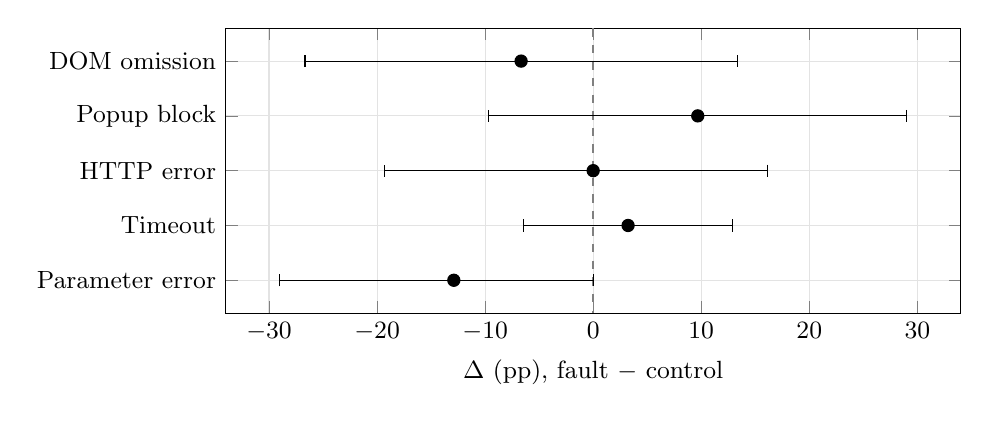
\begin{tikzpicture}
\begin{axis}[
  width=0.9\linewidth, height=5.2cm,
  xlabel={$\Delta$ (pp), fault $-$ control},
  ytick={1,2,3,4,5}, yticklabels={{DOM omission},{Popup block},{HTTP error},{Timeout},{Parameter error}},
  y dir=reverse, ymin=0.4, ymax=5.6,
  xmin=-34, xmax=34, xtick={-30,-20,-10,0,10,20,30},
  grid=major, grid style={gray!22},
  tick label style={font=\small}, label style={font=\small},
]
\draw[gray,dashed,thick] (axis cs:0,0.4) -- (axis cs:0,5.6);
\addplot[only marks, mark=*, mark size=2.2pt, black,
  error bars/.cd, x dir=both, x explicit]
  coordinates {(-6.67,1) -= (20.00,0) += (20.00,0) (9.68,2) -= (19.35,0) += (19.35,0) (0.00,3) -= (19.35,0) += (16.13,0) (3.23,4) -= (9.68,0) += (9.68,0) (-12.90,5) -= (16.13,0) += (12.90,0)};
\end{axis}
\end{tikzpicture}
\caption{Paired risk difference $\Delta$ in official success (fault $-$ control) on native-evaluator pairs, with the percentile bootstrap interval over pair units. Every interval spans zero and no fault survives Holm correction, which is the paper's primary result. Compare Table~\ref{tab:official_native}.}
\label{fig:forest}
\end{figure}

% GENERATED by scripts/paper/figures.py -- do not edit by hand.
\begin{figure}[t]
\centering
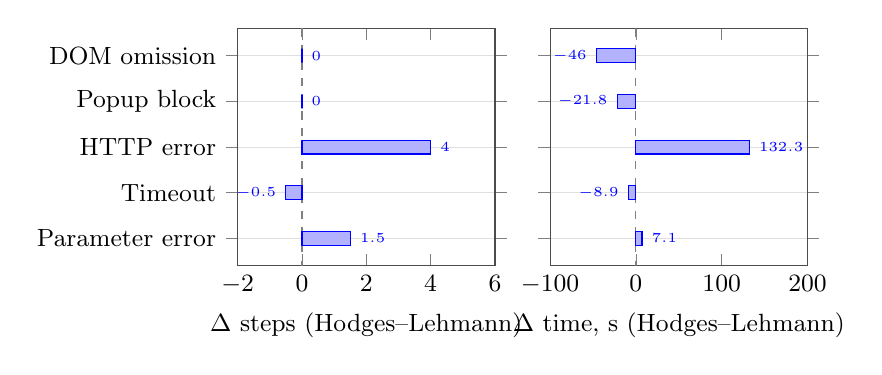
\begin{tikzpicture}
\begin{axis}[name=steps, xbar, bar width=5pt,
  width=0.40\linewidth, xmin=-2, xmax=6,
  ytick={1,2,3,4,5}, y dir=reverse, ymin=0.4, ymax=5.6,
  height=4.6cm,
  tick label style={font=\small}, label style={font=\small},
  nodes near coords, nodes near coords style={font=\tiny},
  ymajorgrids, grid style={gray!25},
  yticklabels={{DOM omission},{Popup block},{HTTP error},{Timeout},{Parameter error}},
  xlabel={$\Delta$ steps (Hodges--Lehmann)},
  fill=gray!60, draw=black!70,
]
\draw[gray,dashed] (axis cs:0,0.4) -- (axis cs:0,5.6);
\addplot coordinates {(0.0,1) (0.0,2) (4.0,3) (-0.5,4) (1.5,5)};
\end{axis}
\begin{axis}[name=time, at={(steps.east)}, anchor=west, xshift=0.7cm,
  xbar, bar width=5pt, width=0.40\linewidth, xmin=-100, xmax=200,
  ytick={1,2,3,4,5}, y dir=reverse, ymin=0.4, ymax=5.6,
  height=4.6cm,
  tick label style={font=\small}, label style={font=\small},
  nodes near coords, nodes near coords style={font=\tiny},
  ymajorgrids, grid style={gray!25},
  yticklabels={},
  xlabel={$\Delta$ time, s (Hodges--Lehmann)},
  fill=gray!60, draw=black!70,
]
\draw[gray,dashed] (axis cs:0,0.4) -- (axis cs:0,5.6);
\addplot coordinates {(-46.0,1) (-21.8,2) (132.3,3) (-8.9,4) (7.1,5)};
\end{axis}
\end{tikzpicture}
\caption{Within-pair process cost on the behavioural matrix. HTTP errors and parameter errors cost the agent steps and time, while DOM omission and popup blocking make it \emph{faster} --- which we read as fault-induced early termination. All five are significant at $p<0.01$ except where noted in Table~\ref{tab:behavior}.}
\label{fig:behavior}
\end{figure}

% GENERATED by scripts/paper/figures.py -- do not edit by hand.
\begin{figure}[t]
\centering
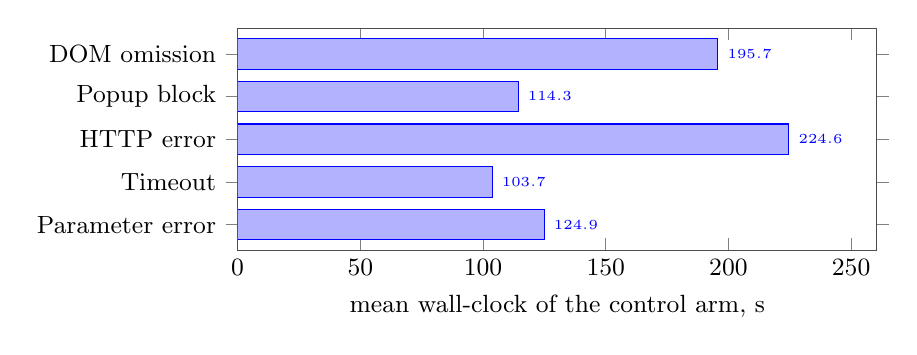
\begin{tikzpicture}
\begin{axis}[
  width=0.8\linewidth, height=4.4cm,
  xbar, bar width=11pt, xmin=0, xmax=260.5,
  ytick={1,2,3,4,5}, y dir=reverse, ymin=0.4, ymax=5.6,
  yticklabels={{DOM omission},{Popup block},{HTTP error},{Timeout},{Parameter error}},
  xlabel={mean wall-clock of the control arm, s},
  tick label style={font=\small}, label style={font=\small},
  nodes near coords, nodes near coords style={font=\tiny},
  fill=gray!55, draw=black!70,
]
\addplot coordinates {(195.7,1) (114.3,2) (224.6,3) (103.7,4) (124.9,5)};
\end{axis}
\end{tikzpicture}
\caption{The noise floor. These five arms are the \emph{same} agent configuration under the clean condition; each is the control half of one fault's pair set. Their means span a factor of 2.17$\times$, so absolute cross-arm timings are dominated by machine-level drift and only within-pair deltas are interpretable.}
\label{fig:noisefloor}
\end{figure}


\section{Supplementary experiment plan}
\label{app:plan}

The staged design that would make the attribution question answerable is released
with this paper. It is ordered by its ability to change the numbers reported here,
not by novelty. \textbf{Stage A} first repairs the evaluator's null-retrieval
schema path and re-evaluates the existing 400 response/HAR pairs offline. Every
frozen row already retains HAR, so repeating the same agent trials would not
remove the schema-triggered fallback; new runs are needed only for artifacts that
the repaired evaluator cannot consume or for deliberately replaced tasks.
\textbf{Stage C} crosses three categorical model levels with three architectures
and three faults. We do not impose an ordinal model-capability contrast: current
provider claims invalidate the earlier Flash--Pro ordering, and the cross-provider
ordering is not independently identified. The confirmatory target is therefore
the omnibus model$\times$architecture interaction followed by preregistered
pairwise and simple-effect contrasts.
\textbf{Stages E and F} add injection-step sensitivity and the repair ablation,
respectively; the former Stage B and D expansions are folded into Stage C. Injection-step sensitivity is
the confound we would press on hardest as a reviewer, since our injector holds the
step fixed throughout. The plan gives exact command lines, the six-worker
wall-clock budget measured from the runs reported here, and the per-trial timings
that size each stage.


\end{document}
